%%%%%%%%%%%%%%%%%% Część III %%%%%%%%%%%%%%%%%

\section{Uczenie nienadzorowane warstwowych sieci neuronowych}

\subsection{Projektowanie i testowanie prostej sieci typu SOM}

\begin{enumerate}
\item \textbf{Utwórz sieć typu mapa odwzorowania cech istotnych (SOM) o wymiarach 5x4 (sugerowanych przez StatsticaNN) dla zbioru IRIS: File|New|Network, potem wybierz Kohonen, Advise, Create.}

\item \textbf{
Otwórz edytor sieci (Edit|Network). Jakiego typu neurony są stosowane w warstwie wyjściowej (okienko z ilustracją sieci to sugeruje) ?}
Stosowane są neurony z radialną funkcją PSP (jak w sieci RBF) oraz pierwiastkową funkcją aktywacji (Act).

\item \textbf{
Zwróć uwagę, jak zdefiniowany jest błąd popełniany przez sieć (Error function) (Suma po wszystkich przykładach odległości pomiędzy przykładem a najbliższym mu wektorem wag neuronów w warstwie wyjściowej => uczenie nienadzorowane!)}

\item \textbf{
Zobacz, jak można zmieniać topologię sieci manewrując parametrem Width dla drugiej warstwy.}

\item \textbf{
Naucz sieć (Train|Kohonen) przy domyślnych ustawieniach parametrów. Zwróć uwagę, że mimo nienadzorowanego charakteru uczenia ma sens wyświetlanie przebiegu błędu.}

\item \textbf{
Co więcej, można używać zbioru weryfikującego i oprzeć na nim warunek stopu. Zbadaj, jak uczy się sieć np. z warunkiem stopu Minimum improvement|Verification = 0.01, Window = 10 (wydaje się to sensowne, bo widać, że minimum lokalne znajdowane jest bardzo szybko i nie ma potrzeby uczyć sieci aż przez 100 epok).}

\item \textbf{
Testowanie sieci. Obejrzyj najpierw, jak „odpowiadają” poszczególne neurony na kolejne przykłady ze zbioru uczącego (Run|Activations). Potem obejrzyj odpowiedzi sieci w diagramie, który zachowuje jej topologię (Run|Topological Map).  Jak grupują się przykłady ?
Zwróć uwagę, że podczas przeglądania przykładów mapą topologiczną, można samemu nazywać przykłady (górne pole bez nazwy) i/lub neurony (dolne pole bez nazwy); działa także prawy przycisk myszki.}
\\Na rysunku \ref{fig:map-iris} przedstawiono mapę topologiczną dla problemu IRIS utworzoną za pomocą sieci SOM. Etykiety przypisano według klasy przykładów najczęściej mapowyanych na dany neuron. Widać, że przestrzenne rozłożenie neuronoów odpowiada podobieństwom między przykładami, do których są one podobne - przykłądy należące do tej samej klasy są zgrupowane.
\begin{figure}[h]
\begin{centering}
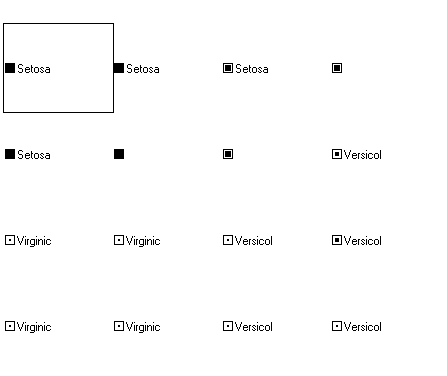
\includegraphics[width=0.6\textwidth]{dane/part3/zad1/map-iris}
\caption{Mapa topologiczna dla dproblemu IRIS\label{fig:map-iris}}
\end{centering}
\end{figure}


\item \textbf{
Poza tym można też obejrzeć statystykę „wygrywania” współzawodnictwa przez poszczególne neurony w poszczególnych podzbiorach (Statistics|Win frequencies).}

\item \textbf{
W podobny sposób naucz i przeanalizuj dla tego samego zbioru sieć o innej topologii (szczególnie ciekawe jest to dla sieci o topologii „jednowymiarowej”, gdzie warstwa wyjściowa ma np. 20 neuronów ułożonych w rzędzie, parametr Width = 1 dla warstwy 2 w edytorze sieci).}
	
\end{enumerate}

\subsection{ Analiza rzeczywistego problemu przy użyciu sieci SOM}

 \paragraph{\textbf{Dane: Zbiór PROTEIN.STA, dostępny lokalnie w katalogu Statistica (Examples). Opisuje on spożycie protein różnego pochodzenia w wybranych krajach Europy. Dane nie są podzielone na klasy decyzyjne.}}
 \paragraph{\textbf{Zbuduj sieć dla tego problemu (sugerowany rozmiar warstwy wyjściowej 4x4 lub nawet 3x3, bo mało przykładów). Naucz ją i przetestuj. Czy da się wyciągnąć i uzasadnić jakieś wnioski dotyczące podobieństwa poszczególnych krajów pod względem spożycia protein? Można, podobnie jak dla IRIS, spróbować z siecią SOM jednowymiarową.}}

\begin{figure}[h]
\begin{centering}
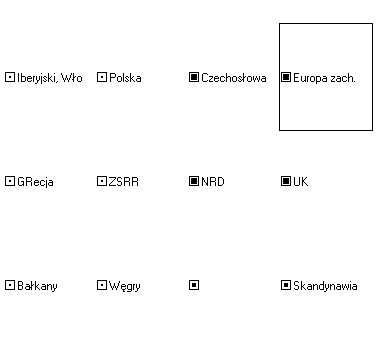
\includegraphics[width=0.6\textwidth]{dane/part3/zad2/proteins12}
\caption{Mapa topologiczna dla problemu PROTEINS. Wierzhołki, do których przypisano więcej niż 2 kraje zostały opisane w poniższy sposób: Europa zachodnia: Austria, Belgia, Francja, Irlandia, Holandia, Szwajcaria, RFN; Bałkany: Albania, Bułgaria, Rumunia, Jugosławia; Skandynawia: Dania, Finlandia, Szwecja, Norwegia; Półwysep Iberyjski: Hiszpania, Portugalia.\label{fig:proteins12}}.
\end{centering}
\end{figure}

Zbudowano sieć som o topologii 4x3. Jak widać na rysunku \ref{fig:proteins12} sieć bardzo dobrze odwzorowuje podobieństwa między państwami (jeśli założyć, że państwa położone blisko siebie cechują się względnie podobnymi nawykami żywieniowymi). Na przykład wszystkie kraje przypisane do wierzchołka o etykiecie "Europa Zachodnia" są rzeczywiście zaliczane do krajów Europy Zachodniej (wg. klasyikacji ONZ). Podobnie było z krajami należącymi do Bałkanów, krajami Skandynawskimi jak i śródziemnomorskimi (półwysep iberyjski i Włochy).

\begin{figure}[h]
\begin{centering}
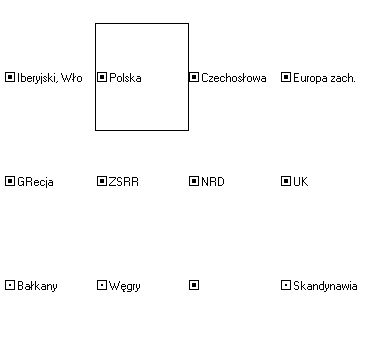
\includegraphics[width=0.6\textwidth]{dane/part3/zad2/polska}
\caption{Mapa topologiczna dla problemu PROTEINS. Pokazana aktywacja dla przykładu Polska.\label{fig:polska}}.
\end{centering}
\end{figure}

Dziwne wydaje się to, że np. Polska, która jako jedyna zajmuje swój wierzchołek, nie jest do niego bardzo podobna - poziom aktywacji jej wierzchołka gdy przypadek "Polska" jest prezentowany na wejście sieci wynosi aż 0.52 i jest zbliżony do poziomu aktywacji wielu innych węzłów (rys. \ref{fig:polska}. Można z tego wysnuć wniosek, że Polska kuchnia nie jest specyficzna, bierze po trochu z innych kuchni.
Inaczej jest np. w przypadku kuchni Norweskiej(rys. \ref{fig:norwegia}):  aktywacja wierzchołka "Skandynawia" jest niska - wynosi 0.38 (czyli przypadek Norwegia jest podobny do tego wierzchołka). Jednocześnie inne wierzchołki są zdecydowanie mniej podobne - najbardziej NRD - 0.67. Można to interpretować w ten sposób, że kuchnia Norweska jest typową kuchnią Skandynawską i jest specyficzna na tle wszystkich kuchni Europejskich.


\begin{figure}[h]
\begin{centering}
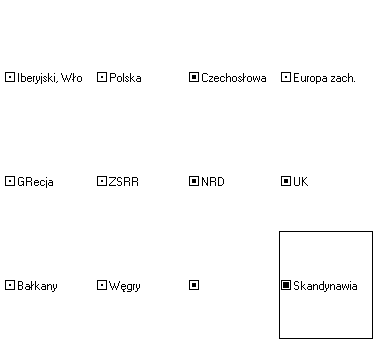
\includegraphics[width=0.6\textwidth]{dane/part3/zad2/norwegia}
\caption{Mapa topologiczna dla problemu PROTEINS. Pokazana aktywacja dla przykładu Norwegia.\label{fig:norwegia}}.
\end{centering}
\end{figure}

\subsection{Projektowanie i testowanie prostej sieci typu SOM}
 \paragraph{\textbf{Zobacz, co się dzieje, gdy opcja "Shuffle cases" jest wyłączona. Sprawdź wpływ parametrów algorytmu uczącego (blisko "skrajnych" wartości parametrów) na przebieg i efekty uczenia.}}
 Dla szybkości uczenia równej 1 wszystkie przykłady zostały przypisane do zaledwie 3 wierzchołków a błąd uczenia był bardzo duży (ok. 0.8). Im mniejsza prędkość uczenia tym mniejszy błąd, ale tym wolniej osiągane warunki stopu. Obserwując wykres błędu sieci i eksperymentując prędkością uczenia można dojść do wniosku, że w przypadku zbioru \emph{PROTEIN} optymalna prędkość wynosi ok 0.1.
Funkcja "Shuffle cases" nie ma istotengo wpływu na błąd uczenia.